\documentclass{article} % For LaTeX2e
\usepackage{cos424,times}
\usepackage{hyperref}
\usepackage{url}
\usepackage{float}
\usepackage{graphicx}


\title{ML1}


\author{
Michael Yitayew\\
Student Researcher\\
\texttt{email} \\
\And
Abhinav Khanna \\
Student Researcher \\
\texttt{akhanna@princeton.edu} \\
}

\newcommand{\fix}{\marginpar{FIX}}
\newcommand{\new}{\marginpar{NEW}}

\begin{document}

\maketitle

\begin{abstract}

\end{abstract}

\section{Introduction}

Music Information Retrieval is a small but growing field, and music genre classification is an important subsection of this field. With the rise of internet services like Pandora, Spotify, and other recommendation systems, the ability for a computer to tag and associate songs has become ever more pressing. Music genre classification is a challenging problem as many songs can be classified under multiple genres. Furthermore, a song is a complex audio wave that must be translated into a digital vector before being classified. This transformation process takes a continuous wave and condenses it down to a vector set, creating some information loss inherent in the problem. In this work, we focus on testing various classification methods, and various features for classifying 30 second music clips into their appropriate genres. This work builds on the work of Tzanetakis and Cook, who published a paper titled "Automatic Musical Genre Classification of Audio Signals," that focuses on the same gtzan dataset that is used in this project. We do a deeper analysis of different classifiers using a similar set of features, analyze the effects of including different features in the classification task, and dissect which genres lead to the highest classification confusion. Through our experiments, we discovered that Blues and Rock are the hardest for our classifiers to isolate from other genres, and thus we report results that both include Blues and Rock as well as exclude those two labels and data subsets. With Blues and Rock, the highest classification accuracy we were able to achieve was 70\%. Without the Blues and Rock data subset, we were able to achieve a 80\% accuracy. 

\section{Related Work}

\section{Methods}
\subsection{Description of data and data processing}
The songs in our study are 30 second clips, and each song was provided as a set of frame-level features for each 20 millisecond frame in the song. ``Frame level features do not encode temporal variation, which is important for genre classification''[3] thus Fisher vectors and exemplars were used to aggregate temporal features into a per song feature vector. 
We performed manual feature selection by observing the discriminant strength of subsets of features on different classifiers; we found MFCC(Mel-Frequency Cepstrum Coefficients) to be the most discriminant feature for genre classification. Other features such as Chroma and Key Strength also slightly improved overall accuracy. 

\subsection{Classification Methods}
We used the following 8 different classifiers; eight are from the SciKitLearn Python Libraries and the Neural Net is from Matlab. 
\begin{enumerate}
    \item \textit{K-nearest-neighbors(KNN)} 
    \item \textit{Logistic Regression with $l_2$ penalty(LR)} using one-vs-rest scheme 
    \item \textit{PCA followed by Logistic Regression (PCALR)}
    \item \textit{Random Forests Classifier}
    \item \textit{PCA followed by Random Forests classifier}
    \item \textit{Support Vector Machine (SVM)} with an exponential kernel function
    \item \textit{Naive Bayes classifier(NB)} using the Multinomial Naive Bayes algorithm
    \item \textit{AdaBoost} with Random Forests as Weak Learners
    \item \textit{NNet Neural Network} from Matlab - A feed forward network with a single hidden sigmoid layer containing 50 neurons and an output softmax layer.
\end{enumerate}
 Decision Trees were not included as Random Forest builds on the Decision Tree data structure, making checking both seem slightly redundant.
\subsection{Evalulation}
We performed stratified 10-fold cross-validation for each classifier. In this procedure, input is divided into 10 random equal size folds. The classifier is then trained on 9 of the folds and tested on a single fold. The accuracy of a classifier is average of the accuracy values achieved when each fold is used as a testing fold.

In addition, we looked at confusion matrices to understand how the error is distributed across labels for each genre category. A confusion matrix is a true labels by predicted labels two dimensional table that counts the number of times a predicted label occurs for a song with a given true label. It provides detailed analysis of where the classifications are missing, and what genres are creating the most misclassification errors.

\section{Results}
We tested the classifiers against a data set containing all ten class labels as well as a data set that did not include Blues and Rock. The following error-rates were achieved at the classifiers' optimal parameter settings against the complete data set. Optimal parameter settings were found by plotting the error-rate vs parameter graph and finding the minimum.  Performance was variable across the classifiers with Neural-Nets, Random Forest and AdaBoost with Random Forests performing the best. \newline
\begin{center}
	\begin{tabular}{ |p{2cm}|p{2.3cm}|}
		\hline
		\multicolumn{2}{|c|}{\textbf{Classification accuracy}} \\
		\hline
		\textbf{Classifier} & \textbf{Error-rate \%} \\
		\hline
		KNN & 42 \\
		LR & 41  \\
		PCALR & 39 \\
		\textbf{RF}    &  \textbf{35} \\
		PCARF & 39 \\
		SVM & 46 \\
		NB & 45 \\
		\textbf{Ada} & \textbf{36} \\
		\textbf{NNet} & \textbf{26} \\
		\hline
	\end{tabular}
\end{center}
In order to better understand what the distribution of misclassifications looked like, we took the top classifiers, and created confusion matrices of their classifications. As you can see in the figure below, the confusion matrix for Random Forest Classifier suggests that Blues and Rock both are often mislabeled as another class, while the rest of the genres appear to be far more accurately classified. This trend reappeared for AdaBoost, and NN based classifiers. In order to verify this, we reran the top classifiers with Blues and Rock removed.
\begin{figure}[!ht]
\begin{center}
\begin{minipage}[b]{0.45\linewidth}
	\caption{Confusion Matrix for Random Forest - With Blues and Rock}
	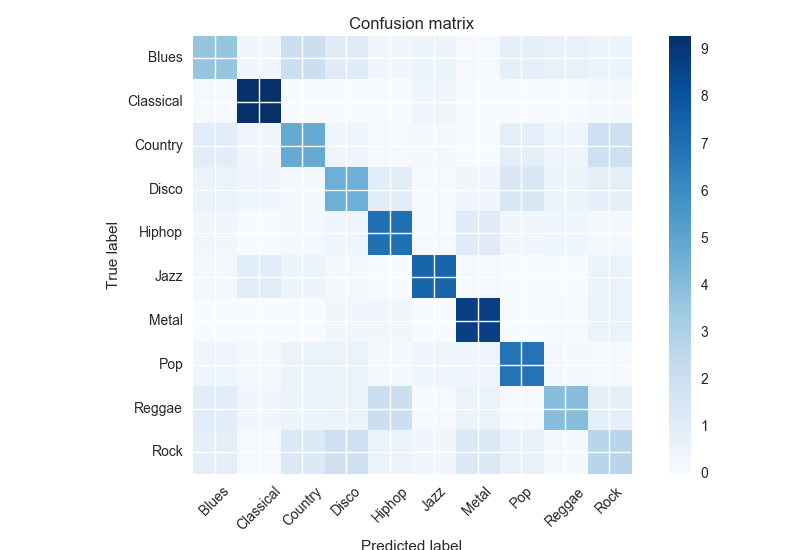
\includegraphics[scale=0.35]{ConfusionMatrix-RandomForest.png}
\end{minipage}
\quad
\begin{minipage}[b]{0.45\linewidth}
	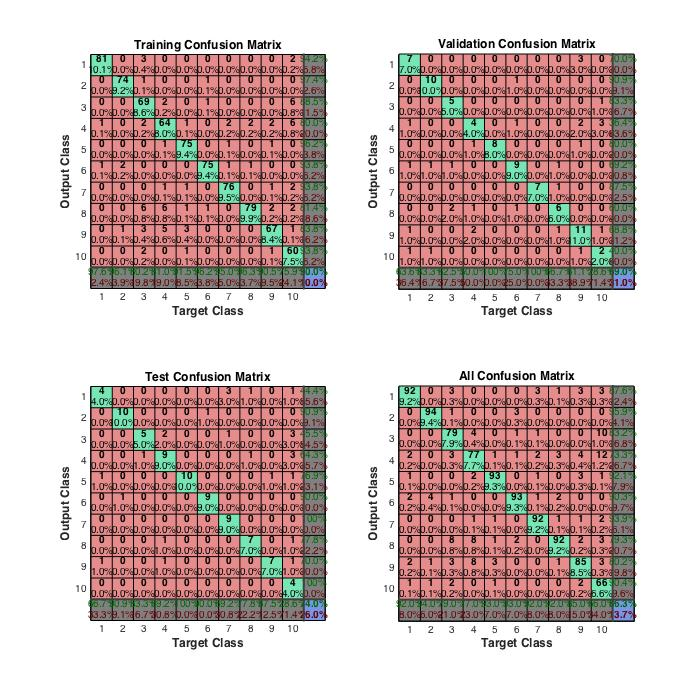
\includegraphics[scale=0.35]{ConfusionMatrix-NN.jpg}
\end{minipage}
\end{center}
\end{figure}
%\textbf{K Nearest-Neighbors}  
%%\begin{figure}[ht!]
%%\centering
%%\includegraphics[width=30mm]{fixed_dome1.jpg}
%%\caption{KNN Confusion Matrix \label{overflow}}
%%\end{figure}
%\vspace{5mm}
%\vspace{5mm}
%\textbf{Logistic Regression}
%\vspace{5mm}
%\vspace{5mm}
%\textbf{PCA + Logisitic Regression} 
%\vspace{5mm}
%\vspace{5mm}
%\textbf{Random Forests}
%\vspace{5mm}
%\vspace{5mm}
%\textbf{PCA + Random Forests} 
%\vspace{5mm}
%\vspace{5mm}
%\begin{tabular}{ |p{2cm}|p{2.3cm}|}
%\hline
%\multicolumn{2}{|c|}{\textbf{Classification accuracy}} \\
%\hline
%\textbf{Classifier} & \textbf{Error-rate \%} \\
%\hline
%KNN & 34 \\
%LR & 41  \\
%PCALR & 39 \\
%RF    &  36 \\
%SVM & 46 \\
%NB & 45 \\
%DT & 0 \\
%Ada & 0 \\
%NNet & 26 \\
%\hline
%\end{tabular}

\section{Discussion and Conclusion}
In this work, we compared 10 classification methods to predict the music genre for a particular 30 second clip after converting the audio signal to a digital vector representation of the features we listed above. After performing manual feature selection and picking the most discriminatory features, we also compared the classification methods with and without Rock and Blues data subset entries from the GTZan data set. Considering the confusion matrices and the classification error rates of the different classifiers with and without the Rock and Blues data subsets, the feed forward neural network performs the best on the data including Blues and Rock subsets, and the data excluding Blues and Rock. Including more Frame-level music features in the Fisher Vector creation process helped yield higher accuracy rates for the neural networks. From a human analysis perspective, it makes sense that the most helpful features for the neural net are features that pertain specifically to musical elements in the song. Its conceivable to imagine that humans also recognize genres based on features of these type.

There are a number of directions we could go to improve this work. Seeing as the Neural Network performed the best on this data set, and that the performance of neural networks increases with the increase in training data, gathering more training data could immensely improve accuracy. Furthermore, different types of neural networks may do a better job at capturing the differences between these classes than the standard feed forward neural network. Recurrent Neural Networks and other custom neural networks may provide increased accuracy and are worth trying. Focusing on better feature extraction, it has been mentioned in literature that instrument details about a given song can be greatly beneficial to genre classification. Adding in instrument recognition to our Fisher Vectors may allow further distinction between these classes. However, because Blues and Rock originate from similar roots and form the basis for many of the other genres, instrument details may not help us resolve the issue of mislabeling Blues and Rock.

\subsubsection*{Acknowledgments}
We would like to acknowledge Princeton University for offering the wonderful COS 424 class that provided us with the opportunity to take on this research. We would also like to thank our Professor, Professor Englehart, and her TA team for providing us with guidance and the tools necessary to make this project happen.

\bibliography{ref}
-Pedregosa F, Varoquaux G, Gramfort A, Michel V, Thirion B, et al. (2011) Scikit-learn: Machine
learning in Python. Journal of Machine Learning Research 12: 2825–2830

\end{document}
